% !TEX root = ../main.tex

\section{Unexpected Results}

  \todo[inline, color=blue!60]{Skriv en introduksjon til "Other Observations"}

\subsection{Association Elements} \label{sec:associationelements}
	An association element are something someone or something you know and can use as a element so the process of remembering can be easier. This is a known technique used in alphanumeric passwords and PIN codes. Alphanumeric passwords are often known to contain personal information like names, dates, and objects close to the user. The same with PIN codes where the the technique of using codes forming a date often occurs. 
  \todo{Kilder} 

  Going through the alphabet, I was able to find 11 patterns having the same visual representation as letters from the alphabet. Out of the 12 letters, 9 patterns had a significant number of appearances in the data set. By iterating through a list of sequences forming a letter, I was able to find 385 out of 3393 patterns in the dataset matching one of the 13 letters in the alphabet. The number of patterns occurred to match a letter from the alphabet constitutes 11.4\% of all patterns in the data set. 

  Figure \ref{fig:associationpatterns} shows the 8 most common patterns having the same visual representation as letters from the alphabet. Beside the letters C, L, M,N, O, S, U and Z, letters like G, J and W also appeared in the data set.

  \clearpage

    \begin{figure}[H]
      \centering
      \vspace{1.5cm}

      \subfigure[The letter C]{
        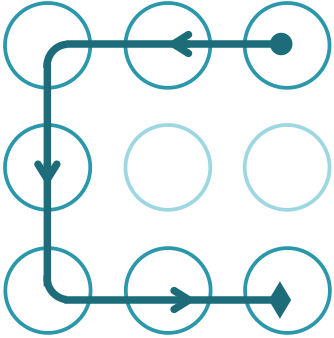
\includegraphics[width=0.27\textwidth]{pics/letters/bokstavenC.png}\hspace{0.6cm}
      }
      \subfigure[The letter L (big)]{
        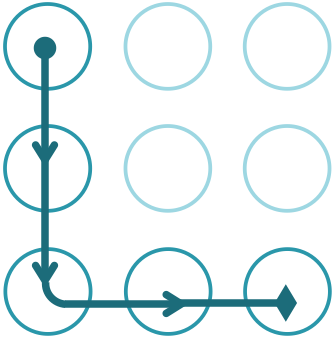
\includegraphics[width=0.27\textwidth]{pics/letters/bokstavenL.png}\hspace{0.6cm}
      }
      \subfigure[The letter L (small)]{
        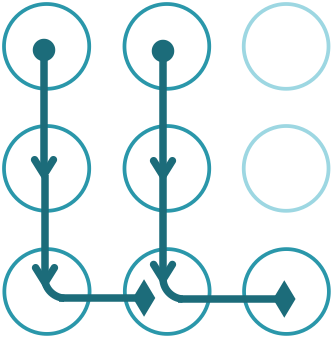
\includegraphics[width=0.27\textwidth]{pics/letters/bokstavenLitenL.png}
      }

      \vspace{0.5cm}

      \subfigure[The letter M]{
        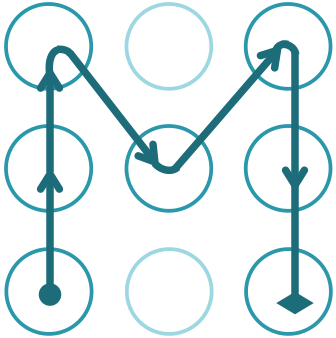
\includegraphics[width=0.27\textwidth]{pics/letters/bokstavenM.png}\hspace{0.6cm}
      }
      \subfigure[The letter N]{
        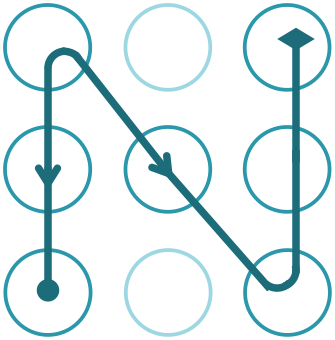
\includegraphics[width=0.27\textwidth]{pics/letters/bokstavenN.png}\hspace{0.6cm}
      }
      \subfigure[The letter O]{
        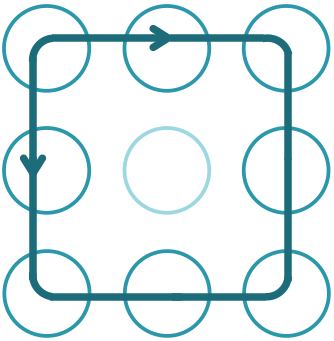
\includegraphics[width=0.27\textwidth]{pics/letters/bokstavenO.png}
      }

      \vspace{0.5cm}

      \subfigure[The letter S]{
        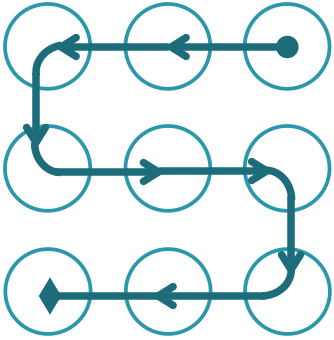
\includegraphics[width=0.27\textwidth]{pics/letters/bokstavenS.png}\hspace{0.6cm}
      }
      \subfigure[The letter U]{
        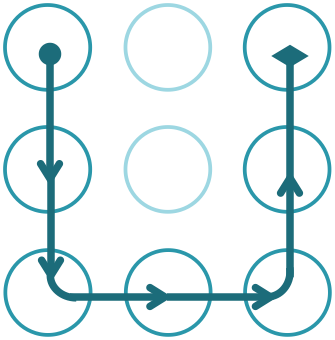
\includegraphics[width=0.27\textwidth]{pics/letters/bokstavenU.png}\hspace{0.6cm}
      }
      \subfigure[The letter Z]{
        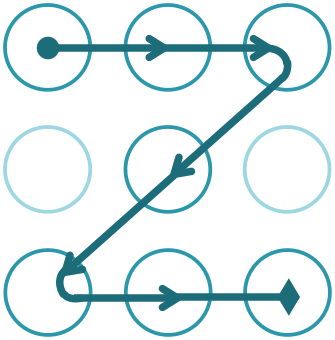
\includegraphics[width=0.27\textwidth]{pics/letters/bokstavenZ.png}
      }

      \vspace{0.5cm}
      \caption{Most frequent patterns forming letters from the alphabet}
      \label{fig:associationpatterns}
    \end{figure}

  \clearpage

\subsection{Bias in the Selection of Start Node}
  
  The starting node of a pattern is a crucial information to have when analyzing patterns because of the properties of a legal pattern. A legal pattern can only visit the same node twice, making the starting point a help for excluding probable patterns.

  Table \ref{tab:startingNode1} is a summary of the likelihood of starting in a particular node for each of the four pattern types. The numbers notation used in the table, 1-3 and T, is a shortcut for the different pattern types shopping account (1), smartphone (2), banking account (3), and training (T). On average, 44\% of all patterns starts in node 1, e.g. the upper-left corner. Summarizing the most common starting points, node 1, 2 and 7, they all together constitutes 73\% of the patterns. 

  %Table: Starting node dist
  \begin{table}[H]
    \centering
    \begin{tabular}{ c || c | c || c | c | c | c }
      \hline
      {\bf Start node} & All & 1,2,3 & 1 & 2 & 3 & T \\ \hline
      1 & 44\% & 42\% & 43\% & 41\% & 42\% & 51\% \\
      3 & 15\% & 15\% & 16\% & 14\% & 13\% & 14\% \\
      7 & 14\% & 14\% & 13\% & 15\% & 14\% & 13\% \\
      2 & 9\%  & 9\%  & 10\% & 9\%  & 8\%  & 7\%  \\
      4 & 6\%  & 7\%  & 6\%  & 7\%  & 7\%  & 6\%  \\
      5 & 4\%  & 4\%  & 4\%  & 4\%  & 4\%  & 3\%  \\
      9 & 4\%  & 4\%  & 3\%  & 3\%  & 5\%  & 3\%  \\
      8 & 2\%  & 3\%  & 2\%  & 3\%  & 3\%  & 2\%  \\
      6 & 2\%  & 2\%  & 2\%  & 2\%  & 3\%  & 2\%  \\ \hline
    \end{tabular}
    \caption{Selection of starting node for all pattern types}
    \label{tab:startingNode1}
  \end{table}

  Figure \ref{fig:startingNode3} is an illustration of the likeliehood of starting in the different nodes. Each node has a number, starting from node 1 in the upper left corner ending up with node number 9 as shown in Figure \ref{fig:startingNode2}. All nodes in Figure \ref{fig:startingNode3} are colored based on the likeliehood of being chosen as a starting point from high to low (green - blue - orange), whereas the green nodes are the most common starting points and orange nodes is the least common starting points.

    %Figure: Staring node for all patterns
  \begin{figure}[H]
    \centering
    \subfigure[Node positions]{
      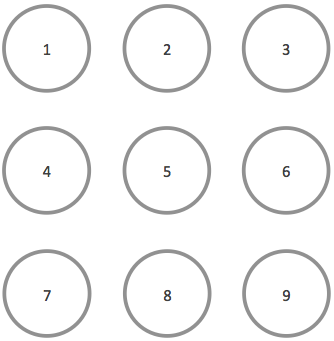
\includegraphics[scale=0.40]{pics/analysis/nodeposition.png}
      \label{fig:startingNode2}
    }
    \hspace{0.7cm}
    \subfigure[Staring node for all pattern types]{
      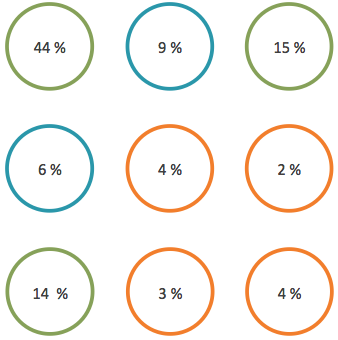
\includegraphics[scale=0.40]{pics/analysis/commonnode.png}
      \label{fig:startingNode3}
    }
    \caption{Node position and likely starting point for all pattern types}
    \label{fig:startingNode4}
  \end{figure}

  How a person are holding a smartphone might impact what nodes are reachable. It was earlier defined two main type people usually interact with their smartphone, e.g. either use one or both hands. When using both hands, one hand are used to hold the phone while the other hand are used for interacting with the screen. When holding the smartphone in one hand, the same hand are used for both holding and interacting with the screen, whereas the thumb are the only finger available when using one hand. Figure \ref{fig:handednessstartingpoint} are showing likelihood of starting nodes from patterns created by respondents with different handedness combined with the two ways of holding a smartphone and finger used. Figure \ref{fig:handednessstartingpoint1} and \ref{fig:handednessstartingpoin2} are looking at right-handed respondents' selection in starting node for patterns created by using either one or two hands. 

  Figure \ref{fig:handednessstartingpoint1} are showing the selection of starting nodes for patterns created by right-handed respondents holding the smartphone in the right hand using the thumb on the same hand for pattern creation. Compared to Figure \ref{fig:startingNode4}, they are similar in the top 3 starting node 1, 3 and 7. Figure \ref{fig:handednessstartingpoin2} are the selection of starting node by right-handed respondents using their left hand holding the smartphone using their right forefinger for pattern creation. The three main starting nodes are 1,3, and 7, and do not have any significant difference from right-handed respondents using one hand. 

  Figure \ref{fig:handednessstartingpoint3} are showing the selection of starting nodes for patterns created by left-handed respondents holding the smartphone in the left hand using the thumb on the same hand for pattern creation. About 54\% of the left-handed respondents using one hand starts in node 1 and 12.5\% starts in node 9, both are corners on the left side of the grid. The starting points in Figure \ref{fig:handednessstartingpoint4}, selected starting points by left-handed respondents using their right hand to hold the smartphone while interacting with the screen using the forefinger on the left hand, are showing about the same distribution of numbers for starting node.

  Looking at the selection of starting node with respect to the handedness of the creator, there are only observed a difference in selection of starting nodes between left- and right-handed respondents. The way of holding the smartphone, either using one or two hands, do not seem to affect the node starting node. 

  \clearpage

  \begin{figure}[H]
    \vspace{1.5cm}
    \centering
    \subfigure[Patterns created by right-handed respondents holding the smartphone in the right hand using the thumb on the same hand]{
      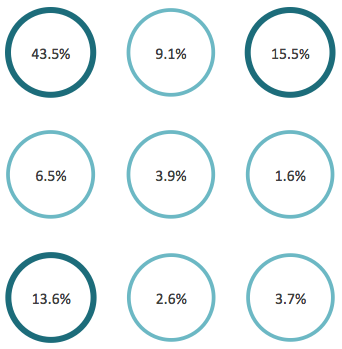
\includegraphics[width=0.45\textwidth]{pics/analysis/RRT.png}
      \label{fig:handednessstartingpoint1}
    }
    \hspace{0.5cm}
    \subfigure[Patterns created by right-handed respondents holding the smartphone in the left hand using the forefinger on the left hand]{
      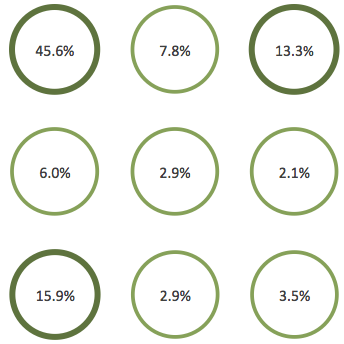
\includegraphics[width=0.45\textwidth]{pics/analysis/RLF.png}
      \label{fig:handednessstartingpoin2}
    }
    \subfigure[Patterns created by left-handed respondents holding the smartphone in the left hand using the thumb on the same hand]{
      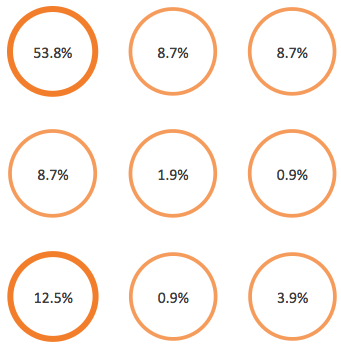
\includegraphics[width=0.45\textwidth]{pics/analysis/LLT.png}
      \label{fig:handednessstartingpoint3}
    }
    \hspace{0.5cm}
    \subfigure[Patterns created by left-handed respondents holding the smartphone in the right hand using the forefinger on the left hand]{
      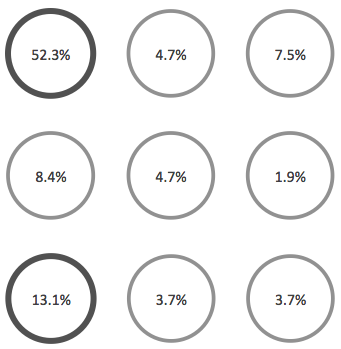
\includegraphics[width=0.45\textwidth]{pics/analysis/LRF.png}
      \label{fig:handednessstartingpoint4}
    }
    \caption{Starting node based on handedness, hand used to hold smartphone, and finger used used when creating patterns}
    \label{fig:handednessstartingpoint}
  \end{figure}

\subsection{3-gram Analysis} \label{sec:3gram}
    
  %Figure: Most common 3-gram to less common 3-gram
  \begin{figure}[H]
    \subfigure{
      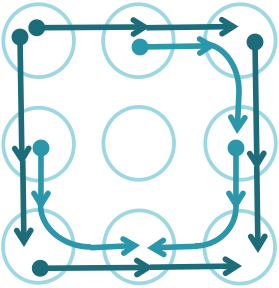
\includegraphics[width=0.31\textwidth]{pics/analysis/3gram1.png}
    }
    \subfigure{
      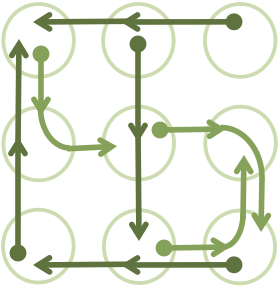
\includegraphics[width=0.31\textwidth]{pics/analysis/3gram2.png}
    }
    \subfigure{
      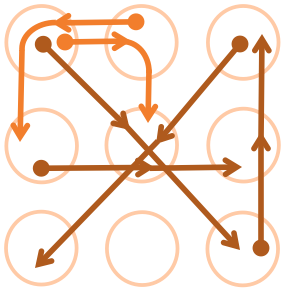
\includegraphics[width=0.31\textwidth]{pics/analysis/3gram3.png}
    }
    \caption{Most common 3-gram to less common 3-gram}
    \label{fig:3gram}
  \end{figure}


